
\chapter{Impossible languages}

% TODO: rewrite opener -- mild AI-tic cluster
% TODO: confirm wordplay -- is "ingrammatical" intentional alongside "antigrammatical"?
Linguists have ventured into the realm of impossible languages, crafting systems that are ungrammatical -- ingrammatical, antigrammatical -- by their very nature. These languages defy the syntactic structures we're familiar with, presenting sentences where words are arranged in random sequences, obliterating any semblance of conventional order. They experiment with grammatical rules based on the numerical position of words or on fully or partially backward sequences. These linguistic constructs stretch the definition of language, inhabiting a space that's scarcely linguistic at all.

\begin{quote}
    In one language, for instance, any string is grammatical as long as its length is prime: any five-word string is in the language, any six-word string is out. Or consider the language where the rule is that any word that occurs in a sentence must occur an even number of times. So, if we use different letters to represent different words, the sequence abbcabcb is grammatical, while bbbcabcb is ungrammatical. \hfill\citep[54]{Sampson1975}
    % TODO: write transitions between Sampson block quotes -- currently stitched with bare \dots
    \dots
    The trouble is that if we use transformations, we can define any kind of language that can be defined at all. I have been talking about ps grammars, transformations, and so on in quite a woolly, intuitive way, but one can make these notions precise and rigorous. If one defines the notion transformational grammar precisely, there is a theorem that any rel can be defined by some transformational grammar. In other words, even the ridiculous case of the prime number language I discussed earlier, which, we agreed, could never occur as a natural language, could be specified by some transformational grammar.
    % TODO: write transitions between Sampson block quotes -- currently stitched with bare \dots
    \dots
    So, although the theory of transformational grammar does not partition the set of rel's into a set of possible and a set of impossible languages, it does impose an ordering on the languages, so that some of the rel's will be relatively easy to describe with transformational notation and other rel's will be much harder to define that way (even though they might be quite easy to define in some other notation system). There are all kinds of notation systems one could imagine, each of which would permit all the rel's to be defined; but, depending which notation system one chooses, one gets a different complexity ordering among the various rel's. If it is empirically true that, in the ordering defined by Chomsky's particular notation system, all the natural languages are relatively near the simple end of the range, then Chomsky's notation must correspond to % TODO: OCR error -- original Sampson 1975 word unrecoverable from this transcription; verify against source
    EJiiirt contingent fact about the nature of natural language. Now it might be the case that there is some feature of the environment, outside the human organism, which forces this structure on the languages that humans use. But % TODO: complete the Sampson quote or trim to a coherent stopping point
    \hfill\citep[56]{Sampson1975}
\end{quote}

% TODO: verify Moro 2016 attribution -- sentences look like quoted material; mark with \enquote{} or convert to block quote if so
To make a negative clause, place \mention{no} after the third word of the clause. The first article of the clause has to agree with the last noun. A closed interrogative clause is formed by inverting the order of the corresponding declarative clause. \citep[55--56]{Moro2016}

% TODO: develop into bridge paragraph
What could this be for?

Sometimes, the best way to clarify something is to imagine what it's not. The hugely influential linguist Noam \textcite{Chomsky1957} believed that some sentences belong to a particular language and other sequences of words don't. But beyond that, he believed the strings that don't can be further subdivided into those that \emph{could} be part of the particular language, and those that simply \emph{couldn't}. To make that more concrete, various ideas have been floated about what these impossible languages might be like.
% EDITORIAL-HPC: Keep the formal-language history, but do not let this chapter
% define grammaticality by generability or statistical probability. Use it to
% show constraints on possible maintenance/projectibility, not to replace the
% detector/coupling account.

For example, in (\ref{ex:even-odd-shuffle}), all the even-numbered words are fronted, preserving their original order. In (\ref{ex:partial-reverse}), a special character is inserted, after which everything is reversed. And in (\ref{ex:tense-hop}), the tense-marker on any verb attaches to the word four positions to the right of the verb (or less if fewer words are available). Figure \ref{fig:imp-possible-languages} puts these and other perturbations on an impossible--possible continuum of these languages.

\ea
    \ea[]{\textit{He cleans all the books on his very messy bookshelf.}\hfill[English]} \label{ex:unperturbed}
    \ex[]{\textit{He all books his messy cleans the on very bookshelf.}\hfill[Even-Odd]}\label{ex:even-odd-shuffle}
    \ex[]{\textit{He cleans all the books on }|\textit{ bookshelf messy very his.}\hfill[Partial reverse]}\label{ex:partial-reverse}
    \ex[]{\textit{He clean all the books on\myuline{s} his very messy bookshelf.}\hfill[Tense hop]}\label{ex:tense-hop}
    \z
\z

\begin{figure}
    \centering
    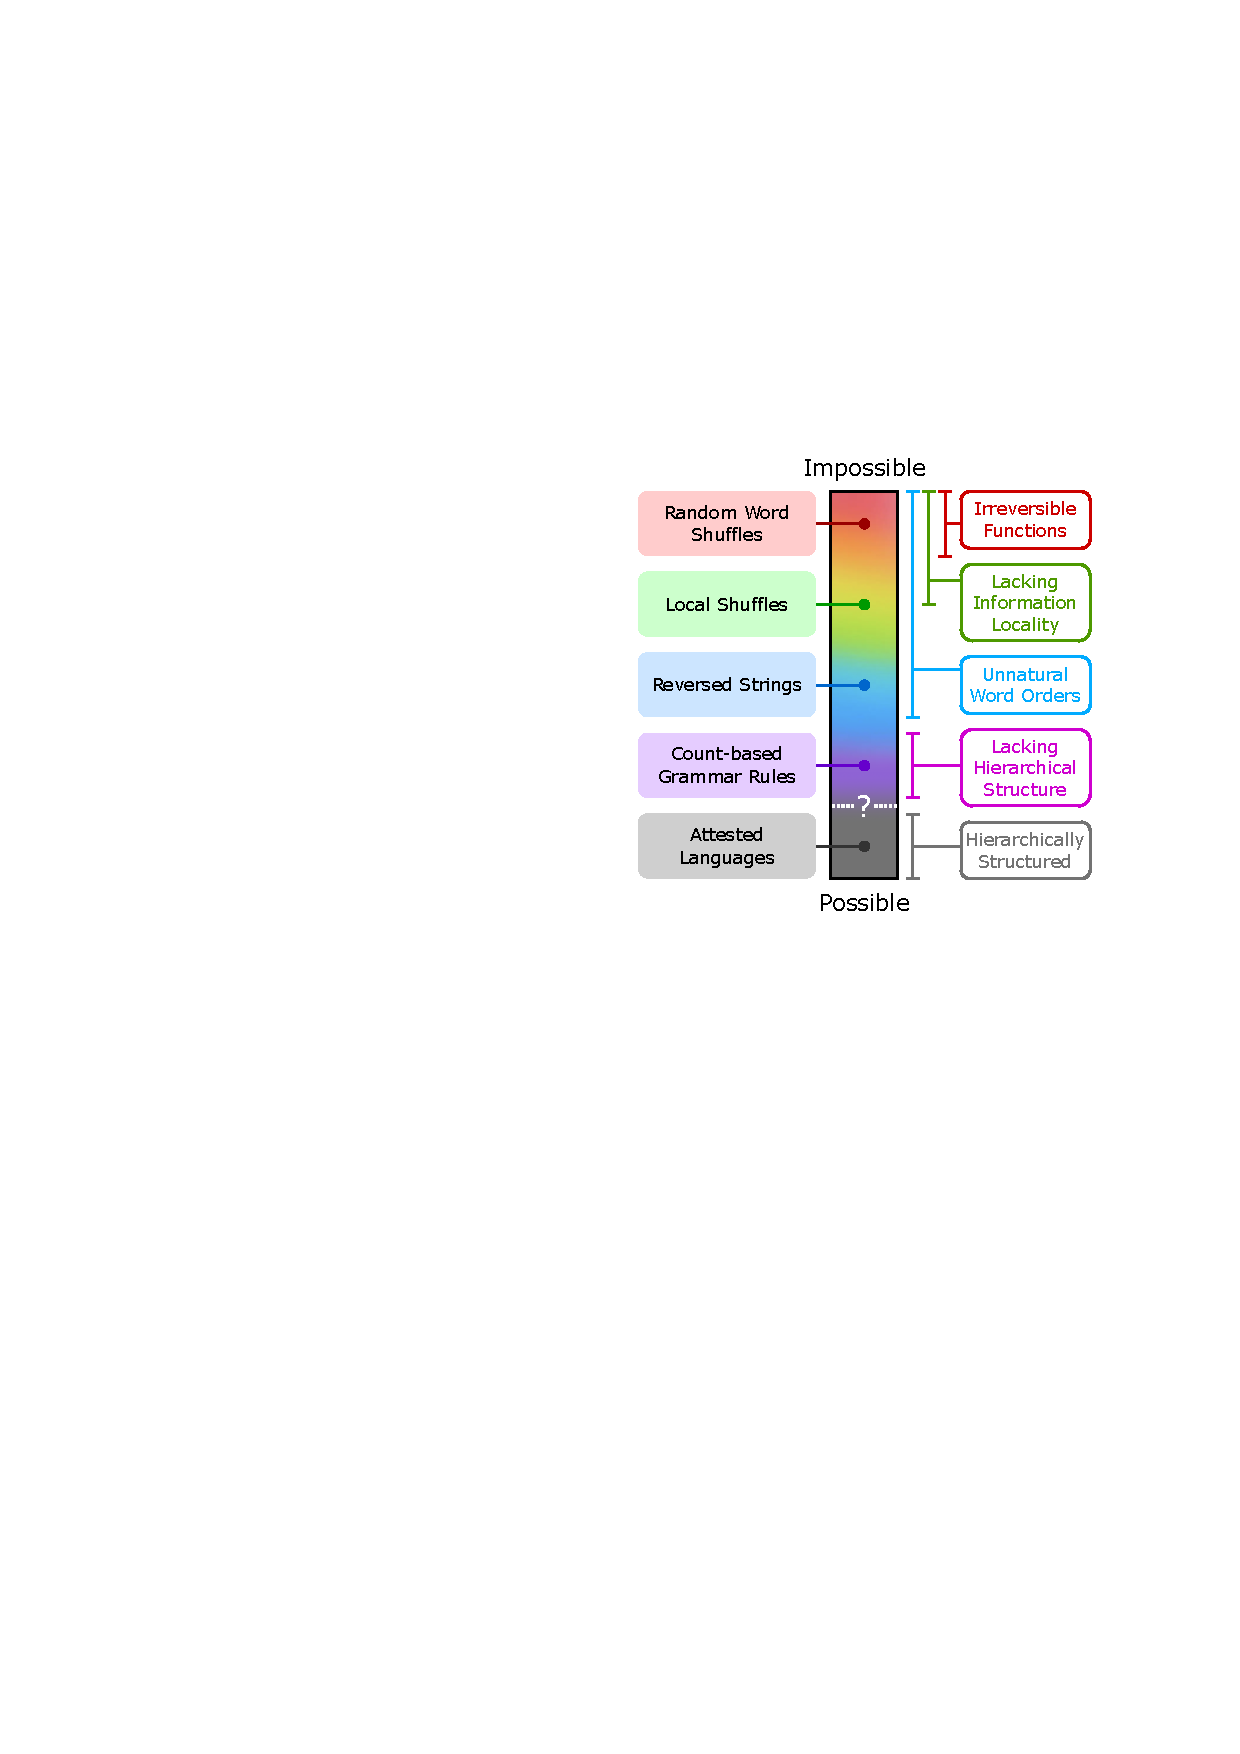
\includegraphics{figures/impossible-languages.pdf}
    % TODO: secure CC-BY downstream-reuse rights for Kallini 2024 Figure 1
    \caption{Partial impossibility continuum of languages based on complexity. Reproduced from \textcite{Kallini2024} Figure 1.}
    \label{fig:imp-possible-languages}
\end{figure}



\section{Remote from English}

Another way to look at the question of why we default to assuming ungrammaticality is caused by grammar, not words, is simply to ask how likely any given sentence is. Back in 1957, Chomsky attempted to illustrate that answering such a question is simply an impossibility with the famous pair of \enquote{sentences} in (\ref{ex:colorless-green-ideas}).

\ea \label{ex:colorless-green-ideas}
    \ea[]{\textit{Colorless green ideas sleep furiously.}}
    \ex[]{\textit{Furiously sleep ideas green colorless.}}
    \z
\z

At the time, he asserted without proof that \enquote{in any statistical model for grammaticalness, these sentences will be ruled out on identical grounds as equally \enquote{remote} from English} \citep[15]{Chomsky1957}. Not so!

Most people find (\ref{ex:colorless-green-ideas}a) to be nonsensical but perfectly grammatical. They realize that the words don't add up to anything they could really make sense of, but that other words might, \textit{colorful green leaves rustle gently}, for instance. Consider, though, that for most people at most times, many sentences seem nonsensical: Werner Heisenberg's observation that \enquote{the more precisely the position [of an electron] is determined, the more imprecisely will the impulse be known, and vice-versa} \citep[5]{Heisenberg1927}, or Martin Heidegger's claim that \enquote{the most thought-provoking thing in our thought-provoking time is that we are still not thinking} \citep{Heidegger1993}, or Friedrich Nietzsche's aphorism, \enquote{when you stare into the abyss, the abyss stares back at you,} \citep{NietzscheBeyondGoodAndEvil}, or Simone de Beauvoir's thought that \enquote{one is not born, but rather becomes, a woman} \citep{DeBeauvoir1949}. Indeed much of what has been said throughout human history might seem meaningless to most of us. These examples illustrate that we're quite familiar with words being put together to mean things we haven't thought or find difficult to think, but that could, with effort, be rendered sensible. And so, though any one of these confounding strings is highly unlikely in itself, the experience of encountering such unexpected collections of words arranged expectedly (or so it would seem) is just a commonplace, not an aberration as Chomsky claimed.

What's truly remote from our experience is seeing strings like (\ref{ex:colorless-green-ideas}b). \citet{Pereira2000} demonstrates this with a simple bigram model. Imagine language as a network of pathways between pairs of words (bigrams). Some are well-worn superhighways between words that often occur together (\textit{and the}), others overgrown trails between words that almost never co-occur (\textit{my the}). Roughly speaking, Pereira looks at likelihood as the total traffic between any two points. Sentences with the most traffic over the shortest distances are more likely in this model. \textit{Colorless green ideas sleep furiously} doesn't take the main streets, but it uses established routes -- people actually do talk about \textit{green ideas}, though \textit{green} means `environmental' here. Meanwhile, \textit{Furiously sleep ideas green colorless} strikes out on its own, forging new paths at each turn. % TODO: verify against Pereira (2000) source
Under this bigram model, the apparently grammatical but meaningless (a) isn't just more likely but roughly 200,000 times more likely than the word salad in (b) \citep[7]{Pereira2000}.

Returning, though, to the difference between lexical meaning and grammatical meaning, it's clear that the words in Chomsky's sentence don't make semantic sense, but the grammar is fully coherent. Its meanings all work.

There's a subject, meaning that the clause is about something -- it has a topic. It also says there's an agent available to perform the action denoted in the predicate. And the subject is an NP, which is conventional.

The noun phrase (NP) has two adjective phrase (AdjP) modifiers, attributing properties from the lexical adjective heads to the head noun. The absence of a determiner means that the NP is indefinite, and nothing in the sentence contradicts this interpretation. The NP is plural, as marked by the morphology of \mention{ideas}. This plurality aligns with the systems of determiners, quantification, and definiteness, all conveying coherent meanings. Even the order of adjectives conforms to standard expectations: a general property adjective (\mention{colorless}) followed by a color adjective (\mention{green}) attributed properties to the entity \mention{ideas}.

The verb phrase (VP) exhibits similar coherence in its grammatical meaning. Placed after the subject, the VP indicates that the subject performs the action denoted by the verb. Specifically, \textit{sleep} requires an Agent role, and the subject NP fulfills this by actively engaging in the action. The present-tense verb form suggests that this situation is a general one, not a particular past or future action, which aligns well with the indefinite nature of the subject.

The verb \textit{sleep} requires a subject, and the grammatical relationship -- that the referent of the subject NP performs the action -- is clear and unviolated. The adverb \textit{furiously}, positioned at the end of the VP, attributes a manner to the action, irrespective of whether sleeping can logically be done furiously. The verb agrees with its plural subject, maintaining grammatical agreement. Crucially, although we might question the plausibility of ideas sleeping (especially furiously), this doesn't violate the grammatical meaning of predication: the action denoted by the verb is attributed to or performed by the subject's referent. The tense marking is appropriate, the word order adheres to English syntax, and all grammatical subsystems operate without contradiction. The sentence's oddness arises entirely from conflicting lexical meanings, not from any failure in grammatical meaning conveyance.

In short, we have sound justifications for our intuition that some sentences are ungrammatical while others are just puzzling, and that, to fix an ungrammatical string such as \textit{two cat}, it makes sense to fix the grammar rather than the choice of words.

The point isn't that probability is grammaticality. It isn't. The point is that remoteness isn't one thing. A string can be remote because its lexical meanings resist each other, because its word order is unlike English, because its dependencies overload us, or because no human community is likely to maintain such a system. The idea of an impossible language begins there.

% TODO: write closing beat -- chapter currently ends without a hand-off to the next
